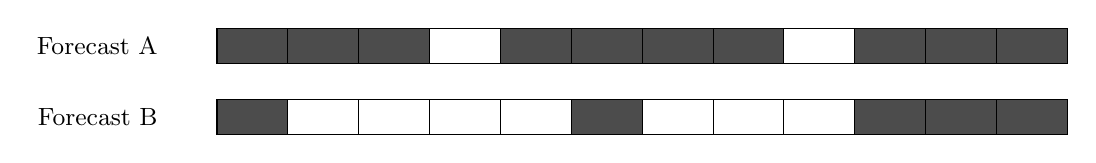
\begin{tikzpicture}[scale=0.9]

% ----------------------------------------------------------
% Forecast A (Higher NSL)
% ----------------------------------------------------------
\node[left] at (-0.7,0.25) {\small Forecast A};

% Covered intervals for Forecast A
\foreach \x in {0,1,2,4,5,6,7,9,10,11} {
    \draw[fill=black!70] (\x,0) rectangle ++(1,0.5);
}

% Shortfall intervals for Forecast A
\foreach \x in {3,8} {
    \draw[fill=white] (\x,0) rectangle ++(1,0.5);
    \draw (\x,0) rectangle ++(1,0.5);
}

% ----------------------------------------------------------
% Forecast B (Lower NSL)
% ----------------------------------------------------------
\node[left] at (-0.7,-0.75) {\small Forecast B};

% Covered intervals for Forecast B
\foreach \x in {0,5,9,10,11} {
    \draw[fill=black!70] (\x,-1) rectangle ++(1,0.5);
}

% Shortfall intervals for Forecast B
\foreach \x in {1,2,3,4,6,7,8} {
    \draw[fill=white] (\x,-1) rectangle ++(1,0.5);
    \draw (\x,-1) rectangle ++(1,0.5);
}

\end{tikzpicture}